\newif\ifshowsolutions
\showsolutionstrue
\documentclass{article}
\usepackage{listings}
\usepackage{amsmath}
\usepackage{subfig}
\usepackage{amsthm}
\usepackage{amsmath}
\usepackage{amssymb}
\usepackage{graphicx}
\usepackage{mdwlist}
\usepackage{geometry}
\usepackage{titlesec}
\usepackage{palatino}
\usepackage{mathrsfs}
\usepackage{fancyhdr}
\usepackage{paralist}
\usepackage{todonotes}
\usepackage{tikz}
\usepackage{float} % Place figures where you ACTUALLY want it
\usepackage{comment} % A hack to toggle sections
\usepackage{ifthen}
\usepackage{mdframed}
\usepackage{verbatim}
\usepackage{listings}
\usepackage{bbm}
\usepackage{upquote} % Prevents backticks replacing single-quotes in verbatim
\usepackage[strings]{underscore}
\usepackage[colorlinks=true]{hyperref}
\usetikzlibrary{positioning,shapes,backgrounds}

\geometry{margin=1in}
\geometry{headheight=2in}
\geometry{top=2in}

\setlength{\marginparwidth}{2.15cm}
\setlength{\parindent}{0em}
\setlength{\parskip}{0.6\baselineskip}

\rhead{}
\lhead{}

% Spacing settings.
\titlespacing\section{0pt}{12pt plus 2pt minus 2pt}{0pt plus 2pt minus 2pt}
\titlespacing\subsection{0pt}{12pt plus 4pt minus 2pt}{0pt plus 2pt minus 2pt}
\titlespacing\subsubsection{0pt}{12pt plus 4pt minus 2pt}{0pt plus 2pt minus 2pt}
\renewcommand{\baselinestretch}{1.15}

% Shortcuts for commonly used operators.
\newcommand{\E}{\mathbb{E}}
\newcommand{\Var}{\operatorname{Var}}
\newcommand{\Cov}{\operatorname{Cov}}
\newcommand{\Bias}{\operatorname{Bias}}
\DeclareMathOperator{\argmin}{arg\,min}
\DeclareMathOperator{\argmax}{arg\,max}

% Do not number subsections and below.
\setcounter{secnumdepth}{1}

% Custom format subsection.
\titleformat*{\subsection}{\large\bfseries}

% Set up the problem environment.
\newcounter{problem}[section]
\newenvironment{problem}[1][]
  {\begingroup
    \setlength{\parskip}{0em}
    \refstepcounter{problem}\par\addvspace{1em}\textbf{Problem~\Alph{problem}\!
    \ifthenelse{\equal{#1}{}}{}{ [#1 points]}:}
  \endgroup}

% Set up the subproblem environment.
\newcounter{subproblem}[problem]
\newenvironment{subproblem}[1][]
  {\begingroup
    \setlength{\parskip}{0em}
    \refstepcounter{subproblem}\par\medskip\textbf{\roman{subproblem}.\!
    \ifthenelse{\equal{#1}{}}{}{ [#1 points]:}}
  \endgroup}

% Set up the teachers and materials commands.
\newcommand\teachers[1]
  {\begingroup
    \setlength{\parskip}{0em}
    \vspace{0.3em} \textit{\hspace*{2em} TAs responsible: #1} \par
  \endgroup}
\newcommand\materials[1]
  {\begingroup
    \setlength{\parskip}{0em}
    \textit{\hspace*{2em} Relevant materials: #1} \par \vspace{1em}
  \endgroup}

% Set up the hint environment.
\newenvironment{hint}[1][]
  {\begin{em}\textbf{Hint: }}
  {\end{em}}


% Set up the solution environment.
\ifshowsolutions
  \newenvironment{solution}[1][]
    {\par\medskip \begin{mdframed}\textbf{Solution~\Alph{problem}#1:} \begin{em}}
    {\end{em}\medskip\end{mdframed}\medskip}
  \newenvironment{subsolution}[1][]
    {\par\medskip \begin{mdframed}\textbf{Solution~\Alph{problem}#1.\roman{subproblem}:} \begin{em}}
    {\end{em}\medskip\end{mdframed}\medskip}
\else
  \excludecomment{solution}
  \excludecomment{subsolution}
\fi




%%%%%%%%%%%%%%%%%%%%%%%%%%%%%%
% HEADER
%%%%%%%%%%%%%%%%%%%%%%%%%%%%%%

\chead{
  {\vbox{
      \vspace{2mm}
      \large
      Machine Learning \& Data Mining \hfill
      Caltech CS/CNS/EE 155 \hfill \\[1pt]
      Set 4\hfill
      February $2^\text{nd}$, 2022 \\
    }
  }
}

\begin{document}
\pagestyle{fancy}



%%%%%%%%%%%%%%%%%%%%%%%%%%%%%%
% POLICIES
%%%%%%%%%%%%%%%%%%%%%%%%%%%%%%

% \section*{Policies}
% \begin{itemize}
%   \item \textbf{Due 9 PM, February $2^\text{nd}$}, via Gradescope.
%   \item You are free to collaborate on all of the problems, subject to the collaboration policy stated in the syllabus.
%   \item In this course, we will be using Google Colab for code submissions. You will need a Google account.
%   \item This set uses PyTorch, a Python package for neural networks. We recommend using Google Colab, which comes with PyTorch already installed. There will be a PyTorch recitation to help you get started.
% \end{itemize}

% \section*{Submission Instructions}
% \begin{itemize}
% \item Submit your report as a single .pdf file to Gradescope (entry code 7426YK), under "Set 4 Report". 
% 	\item In the report, \textbf{include any images generated by your code} along with your answers to the questions.
% 	\item Submit your code by \textbf{sharing a link in your report} to your Google Colab notebook for each problem (see naming instructions below). Make sure to set sharing permissions to at least "Anyone with the link can view". \textbf{Links that can not be run by TAs will not be counted as turned in.} Check your links in an incognito window before submitting to be sure. 
% 	\item For instructions specifically pertaining to the Gradescope submission process, see \url{https://www.gradescope.com/get_started#student-submission}.
% \end{itemize}

% \section*{Google Colab Instructions}
% For each notebook, you need to save a copy to your drive.
% \begin{enumerate}
% 	\item Open the github preview of the notebook, and click the icon to open the colab preview.
% 	\item On the colab preview, go to File $\rightarrow$ Save a copy in Drive.
% 	\item Edit your file name to “lastname_firstname_set_problem”, e.g.”yue_yisong_set4_prob2.ipynb”
% \end{enumerate}

% \section*{TA Office Hours}
% \begin{itemize}
%     \item \textbf{Megan Tjandrasuwita [Question 1 and Question 2]}
%         \begin{itemize}
%             \item Monday 1/31: 3:00 pm - 4:00 pm (Annenberg North Lawn Tent), Tuesday, 2/1: 5:00 pm - 6:00 pm (Zoom)
%         \end{itemize}
%     \item \textbf{Pantelis Vafidis [Question 3]}
%         \begin{itemize}
%             \item Monday, 1/31: 6:00 pm - 8:00 pm (Zoom)
%         \end{itemize}
% \end{itemize}

%%%%%%%%%%%%%%%%%%%%%%%%%%%%%%
% PROBLEM 1
%%%%%%%%%%%%%%%%%%%%%%%%%%%%%%

\newpage
\section{Deep Learning Principles [35 Points]}
\materials{lectures on deep learning}

    For problems A and B, we'll be utilizing the \href{http://playground.tensorflow.org/}{Tensorflow Playground} to visualize/fit a neural network.

\begin{problem}[5]
    Backpropagation and Weight Initialization Part 1
\end{problem}

Fit the neural network at \href{http://playground.tensorflow.org/#activation=relu&batchSize=10&dataset=circle&regDataset=reg-plane&learningRate=0.03&regularizationRate=0&noise=0&networkShape=4,2&seed=0.65409&showTestData=false&discretize=false&percTrainData=50&x=true&y=true&xTimesY=false&xSquared=false&ySquared=false&cosX=false&sinX=false&cosY=false&sinY=false&collectStats=false&problem=classification&initZero=false&hideText=false}{this link} for about 250 iterations, and then do the same for the neural network at  \href{http://playground.tensorflow.org//\#activation=relu&batchSize=10&dataset=circle&regDataset=reg-plane&learningRate=0.03&regularizationRate=0&noise=0&networkShape=4,2&seed=0.6&showTestData=false&discretize=false&percTrainData=50&x=true&y=true&xTimesY=false&xSquared=false&ySquared=false&cosX=false&sinX=false&cosY=false&sinY=false&collectStats=false&problem=classification&initZero=true&hideText=false}{this link}.  Both networks have the same architecture and use ReLU activations.  The only difference between the two is how the layer weights were initialized -- you can examine the layer weights by hovering over the edges between neurons.

Give a mathematical justification, based on what you know about the backpropagation algorithm and the ReLU function, for the difference in the performance of the two networks.

\begin{solution}
    One of the networks is initialized with random weights and the other is initialized with 0 weight. In order to improve the performance of the network during training, the backpropagation algorithm computes the gradient of the loss with respect to the weights of each layer and uses the gradient to adjust the weights in the network. One of the terms in the chain rule decomposition of the gradient is $\partial s^{(L)} / \partial W^{(L)}$. However, if $\sigma(w \cdot x) = \sigma(s^{(L)}) = x^{(L)}$ is the ReLU function, the gradient $\partial s^{(L)} / \partial W^{(L)}$ vanishes at $W = 0$, since this is simply $\partial s^{(L)} / \partial W^{(L)} = x^{(L-1)}$. Since all $s$ are 0 (due to $W = 0$) and the ReLU function is 0 at input 0, all $x$ are 0 as well. Since for each set of weights $W^{(L)}$ we compute the gradient with $\partial s^{(L)} / \partial W^{(L)}$ in the product, which is 0, all gradients with respect to the weights are 0. Thus, no changes occur when backpropagation is used during gradient descent.
\end{solution}

\newpage

\begin{problem}[5]
    Backpropagation and Weight Initialization Part 2
\end{problem}
Reset the two demos from part i (there is a reset button to the left of the ``Run'' button), change the activation functions of the neurons to sigmoid instead of ReLU, and train each of them for 4000 iterations.

Explain the differences in the models learned, and the speed at which they were learned, from those of part i in terms of the backpropagation algorithm and the sigmoid function.

\begin{solution}
    After changing the model's activation function from ReLU to sigmoid, the boundary learned by the randomly initialized model was much smoother and less polygonal. This is because the sigmoid function is a smoother activation function than the ReLU function, and thus creates smoother and less linear boundaries.
    
    The model with random initialization converged after around 1000 iterations, after which the test and training losses decreased slowly. This is much slower than the ReLU model, which converged after around 200 iterations. The gradients for the sigmoid activation function are smaller than that of the ReLU activation function for most values, so each iteration of backpropagation using the ReLU function changed the weights more than sigmoid, thus causing the ReLU model to converge more quickly.

    For the model with 0 weight initialization, the model with sigmoid activiation eventually learned a boundary after around 3500 iterations, compared to no boundary learned using the ReLU function, but it was still not very accurate. The weights of this model slowly decreased, but since the gradient of the sigmoid activation function is small, it modified the weights very slowly. Additionally, since the weights were all initialized to the same value, the gradient computed was the same across all weights, so they all changed to the same values. This led to a model where each layer's weights are the same, so although the model has several hidden units, each hidden unit has the same weight, so the hidden layers behave like linear classifiers.
\end{solution}

\newpage

\problem \textbf{[10 Points]}

When training any model using SGD, it's important to shuffle your data to avoid correlated samples. To illustrate one reason for this that is particularly important for ReLU networks, consider a dataset of 1000 points, 500 of which have positive (+1) labels, and 500 of which have negative (-1) labels. What happens if we train a fully-connected network with ReLU activations using SGD, looping through all the negative examples before any of the positive examples? (Hint: this is called the ``dying ReLU'' problem.)

\begin{solution}
    If we train with only negative examples, the weights and biases will adjust so that the input to the final activation, $s^{(L)}$, is negative. In order to guarantee this, the network will either introduce large negative weights in the final layer $W^{(L)}$ (the inputs to this layer are non-negative since the output of ReLU are non-negative), or introduce a large negative bias to guarantee that $s^{(L)}$ is negative. Then, when a positive example is used, the model will still have negative weights, so the gradient of the ReLU function $\partial x^{(L)} / \partial s^{(L)}$ is computed with $s^{(L)} < 0$. In this region, the ReLU function has gradient 0, so the overall gradient computed with respect to all weights using the chain rule (which includes the $\partial x^{(L)} / \partial s^{(L)}$ term) is 0. Thus, backpropagation does not change the weights and the model cannot learn.
\end{solution}

\newpage

\problem Approximating Functions Part 1 \textbf{[7 Points]}

Draw or describe a fully-connected network with ReLU units that implements the OR function on two 0/1-valued inputs,  $x_1$ and $x_2$.  Your networks should contain the minimum number of hidden units possible.  The OR function $\text{OR}(x_1, x_2)$ is defined as:
\begin{gather*}
\text{OR}(1, 0) \geq 1 \\
\text{OR}(0, 1) \geq 1 \\
\text{OR}(1, 1) \geq 1 \\
\text{OR}(0, 0) = 0
\end{gather*}

Your network need only produce the correct output when $x_1 \in \{0, 1\}$ and $x_2 \in \{0, 1\}$ (as described in the examples above).

\begin{solution}
    We can do this with 1 hidden unit. Let the first weight vector be $\langle 0, 1, 1 \rangle$. With this weight vector, if one of $x_1, x_2$ is 1, then $s^{(1)} = 1$, and if both are 1, then $s^{(1)} = 2$. Then, after activation, $x^{(1)} = 1$ or $x^{(1)} = 2$ for those respective cases, which satisfies the OR function. In the case where $x_1, x_2 = 0, 0$, then $s^{(1)} = 0$, so $x^{(1)} = 0$, as desired.

    \begin{figure}[H]
        \centering
        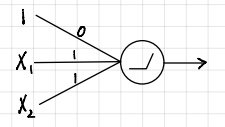
\includegraphics[width=0.6\textwidth]{images/1d.png}
        \caption{Illustration of fully-connected network for the OR function.}
        \label{fig:1d}
    \end{figure}
\end{solution}

\problem Approximating Functions Part 2 \textbf{[8 Points]}

What is the minimum number of fully-connected layers (with ReLU units) needed to implement an XOR of two 0/1-valued inputs $x_1, x_2$? Recall that the XOR function is defined as:
\begin{gather*}
\text{XOR}(1, 0) \geq 1 \\
\text{XOR}(0, 1) \geq 1 \\
\text{XOR}(0, 0) = \text{XOR}(1, 1) = 0
\end{gather*}

For the purposes of this problem, we say that a network $f$ computes the XOR function if $f(x_1, x_2) = \text{XOR}(x_1, x_2)$ when $x_1 \in \{0, 1\}$ and $x_2 \in \{0, 1\}$ (as described in the examples above).

Explain why a network with fewer layers than the number you specified cannot compute XOR.


\begin{solution}
    We can do this with 2 hidden units and 1 output unit. In total, we need 1 hidden layer and one output layer to compute the XOR function. Let the weight matrices be
    \[
        W^{(1)} = \begin{bmatrix}
            -1 & 1\\
            1 & -1\\
            1 & -1
        \end{bmatrix},
        W^{(2)} = \begin{bmatrix}
            1\\ -1\\ -1
        \end{bmatrix}
    \]
    Intuitively, the weight matrices produce a hidden unit with positive value 1 if the inputs $x_1, x_2$ are either both 1 or both 0. Then, the bias in the second layer produces a positive output if neither of the hidden units have value 1. Thus, the network produces the desired outputs.
    
    \begin{center}
        \begin{tabular}{|c|c|c|c|}
            \hline
            $x_1$ & $x_2$ & $s^{(1)}$ & $s^{(2)}$\\
            \hline
            $1$ & $1$ & $\langle 1, 0 \rangle$ & $0$\\
            $1$ & $0$ & $\langle 0, 0 \rangle$ & $1$\\
            $0$ & $1$ & $\langle 0, 0 \rangle$ & $1$\\
            $0$ & $0$ & $\langle 0, 1 \rangle$ & $0$\\
            \hline
        \end{tabular}
    \end{center}
    
    \begin{figure}[H]
        \centering
        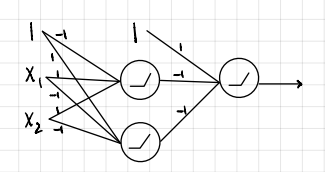
\includegraphics[width=0.6\textwidth]{images/1e.png}
        \caption{Illustration of fully-connected network for the XOR function.}
        \label{fig:1e}
    \end{figure}

    The reason that a network with less hidden units cannot compute the XOR function is because the dataset for the XOR function is not linearly separable. The XOR function requires at least 2 lines to separate, and each hidden unit of a single layer neural network acts as a linear model that separates the data. Therefore, a network with a single hidden unit would only be able to produce a linear classifier, which is not sufficient to separate the XOR function.
\end{solution}


% problem 2
\newpage
\section{Depth vs Width on the MNIST Dataset  [25 Points, 6 EC Points]}

\textit{Relevant Materials: Lectures on Deep Learning}

MNIST is a classic dataset in computer vision. It consists of images of handwritten digits (0 - 9) and the correct digit classification. In this problem you will implement a deep network using PyTorch to classify MNIST digits. Specifically, you will explore what it really means for a network to be "deep", and how depth vs. width impacts the classification accuracy of a model. You will be allowed at most $N$ hidden units, and will be expected to design and implement a deep network that meets some performance baseline on the MNIST dataset.

\medskip

\problem \textbf{Installation} \textbf{[2 Points]}


Before any modeling can begin, PyTorch must be installed. PyTorch is an automatic differentiation framework that is widely used in machine learning research.  We will also need the \textbf{torchvision} package, which will make downloading the MNIST dataset much easier. 

If you use Google Colab (recommended), you won't need to install anything.

If you want to run PyTorch locally, follow the steps on \\
\url{https://pytorch.org/get-started/locally/#start-locally}. Select the 'Stable' build and your system information. We highly recommend using Python 3.6+. CUDA is not required for this class, but it is necessary if you want to do GPU-accelerated deep learning in the future.

Write down the version numbers for both \textbf{torch} and \textbf{torchvision} that you have installed. On Google Colab, you can find version numbers by running: \begin{verbatim}!pip list | grep torch\end{verbatim}

\begin{solution}
    \href{https://colab.research.google.com/drive/1X0ubndLxRFhZ5_vloQmLcP0539Q6jQqB?usp=sharing}{Code link}

    https://colab.research.google.com/drive/1X0ubndLxRFhZ5_vloQmLcP0539Q6jQqB?usp=sharing

    \begin{itemize}
        \item torch version: 1.10.0+cu111
        \item torchvision version: 0.11.1+cu111
    \end{itemize}
\end{solution}

\newpage

\problem \textbf{The Data} \textbf{[5 Points]}

Load the MNIST dataset using torchvision; see the problem 2 sample code for how.

Image inputs in PyTorch are generally 3D tensors with the shape (no. of channels, height, width). Examine the input data. What are the height and width of the images? What do the values in each array index represent?  How many images are in the training set? How many are in the testing set? You can use the \textbf{imshow} function in matplotlib if you'd like to see the actual pictures (see the sample code).

\begin{solution}
    The shape of the image is $[1, 28, 28]$, so the height and width of the images is $28 \times 28$ pixels. Each index in the array represents a single intensity value for the pixel. In color images, the 3 channels represent the intensity of RGB values for each pixel, but since the dataset is greyscale, each of the $1 \times 28 \times 28$ array indices map directly to pixel intensities at each $(x,y)$ location in the image.

    There are 60000 images in the training dataset and 10000 in the test dataset.

    \begin{figure}[H]
        \centering
        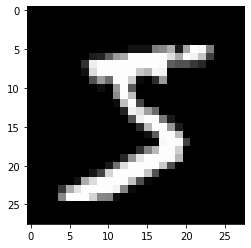
\includegraphics[width=0.3\textwidth]{images/2b.png}
        \caption{Example from MNIST dataset}
        \label{fig:2b}
    \end{figure}
\end{solution}

 \problem \textbf{Modeling Part 1} \textbf{[10 Points]}

 Using PyTorch's "Sequential" model class, build a deep network to classify the handwritten digits. You may \textbf{only} use the following layers:

 \begin{itemize}
    \item \textbf{Flatten:} Flattens any tensor into a single vector
    \item \textbf{Linear:} A fully-connected layer
    \item \textbf{ReLU (activation):} Sets negative inputs to 0
    \item \textbf{Softmax (activation):} Rescales input so that it can be interpreted as a (discrete) probability distribution.
    \item \textbf{Dropout:} Takes some probability and at every iteration sets weights to zero at random with that probability (effectively regularization)
\end{itemize}

A sample network with 20 hidden units is in the sample code file. (Note: You may use multiple layers as long as the total number of hidden units are within the limit. Activations, Dropout, and your last Linear layer do not count toward your hidden unit count, because the final layer is ``observed'' and not \emph{hidden}.)

Use categorical cross entropy as your loss function. There are also a number of optimizers  you can use (an optimizer is just a fancier version of SGD), and feel free to play around with them, but RMSprop and Adam are the most popular and will probably work best. You also should find the batch size and number of epochs that give you the best results (default is batch size = 32, epochs=10).

Look at the sample code to see how to train your model. You can tinker with the network architecture by swapping around layers and parameters.

\textbf{Your task}. Using at most 100 hidden units, build a network using only the allowed layers that achieves test accuracy of at least 0.975. Turn in the code of your model as well as the best test accuracy that it achieved.



\begin{solution}
    The code link contains cells with all 3 models for parts C, D, E.

    \href{https://colab.research.google.com/drive/1X0ubndLxRFhZ5_vloQmLcP0539Q6jQqB?usp=sharing}{Code link}

    https://colab.research.google.com/drive/1X0ubndLxRFhZ5_vloQmLcP0539Q6jQqB?usp=sharing

    A fully connected network consisting of a layer of 60 hidden units, ReLU activation, $0.1$ probability dropout, a layer of 40 hidden units, and ReLU activation achieved a highest test accuracy of $97.66\%$ or $\boxed{0.9766}$ when trained for 20 epochs with a batch size of 32 and learning rate $1 \times 10^{-3}$.

    \begin{verbatim}
        model = nn.Sequential(
            nn.Flatten(),  
            nn.Linear(784, 60),
            nn.ReLU(),
            nn.Dropout(0.1),
            nn.Linear(60, 40),
            nn.ReLU(),
            nn.Linear(40, 10)
        )
    \end{verbatim}
\end{solution}

\newpage

\problem \textbf{Modeling Part 2} \textbf{[8 Points]}

Repeat problem C, except that now you may use 200 hidden units and must build a model with at least 2 hidden layers that achieves test accuracy of at least 0.98.

\begin{solution}
    The code link contains cells with all 3 models for parts C, D, E.

    \href{https://colab.research.google.com/drive/1X0ubndLxRFhZ5_vloQmLcP0539Q6jQqB?usp=sharing}{Code link}

    https://colab.research.google.com/drive/1X0ubndLxRFhZ5_vloQmLcP0539Q6jQqB?usp=sharing

    A fully connected network consisting of a layer of 120 hidden units, ReLU activation, $0.1$ probability dropout, a layer of 80 hidden units, and ReLU activation achieved a highest test accuracy of $98.11\%$ or $\boxed{0.9811}$ when trained for 20 epochs with a batch size of 64 and learning rate $1 \times 10^{-3}$.

    \begin{verbatim}
        model = nn.Sequential(
            nn.Flatten(),
            nn.Linear(784, 120),
            nn.ReLU(),
            nn.Dropout(0.1),
            nn.Linear(120, 80),
            nn.ReLU(),
            nn.Dropout(0.1),
            nn.Linear(80, 10)
        )
    \end{verbatim}
\end{solution}

\newpage

\problem \textbf{Modeling Part 3} \textbf{[6 EC Points]}

Repeat problem C, except that now you may use 1000 hidden units and must build a model with at least 3 hidden layers that achieves test accuracy of at least 0.983.

\begin{solution}
    The code link contains cells with all 3 models for parts C, D, E.

    \href{https://colab.research.google.com/drive/1X0ubndLxRFhZ5_vloQmLcP0539Q6jQqB?usp=sharing}{Code link}

    https://colab.research.google.com/drive/1X0ubndLxRFhZ5_vloQmLcP0539Q6jQqB?usp=sharing

    A fully connected network consisting of
    \begin{itemize}
        \item 400 hidden units with ReLU activation and 0.1 probability dropout
        \item 300 hidden units with ReLU activation and 0.1 probability dropout
        \item 300 hidden units with ReLU activation and 0.1 probability dropout
    \end{itemize}
    achieved a highest test accuracy of $98.43\%$ or $\boxed{0.9843}$ when trained for 20 epochs with a batch size of 64 and learning rate $1 \times 10^{-3}$.

    \begin{verbatim}
        model = nn.Sequential(
            nn.Flatten(),
            nn.Linear(784, 400),
            nn.ReLU(),
            nn.Dropout(0.1),
            nn.Linear(400, 300),
            nn.ReLU(),
            nn.Dropout(0.1),
            nn.Linear(300, 300),
            nn.ReLU(),
            nn.Dropout(0.1),
            nn.Linear(300, 10)
        )
    \end{verbatim}
\end{solution}

\newpage
% problem 3
\section{Convolutional Neural Networks  [40 Points]}
\textit{Relevant Materials: Lecture on CNNs}

\problem Zero Padding \textbf{[5 Points]}

Consider a convolutional network in which we perform a convolution over each $8 \times 8$ patch of a $20 \times 20$ input image. It is common to zero-pad input images to allow for convolutions past the edges of the images. An example of zero-padding is shown below:

\begin{center}
    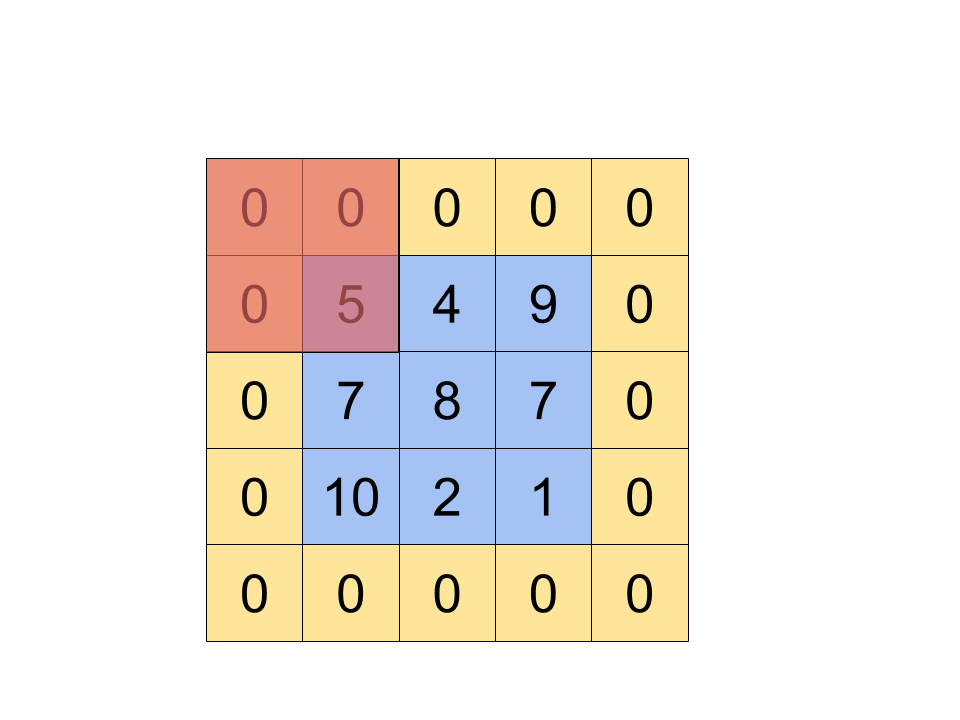
\includegraphics[width=.49\textwidth]{Plots/ConvolutionExample.png}
\end{center}
\begin{small}
Figure: A convolution being applied to a $2 \times 2$ patch (the red square) of a $3 \times 3$ image that has been zero-padded to allow convolutions past the edges of the image.
\end{small}

What is one benefit and one drawback to this zero-padding scheme (in contrast to an approach in which we only perform convolutions over patches entirely contained within an image)?

\begin{solution}
    One benefit of using 0 padding is that we can preserve the shape and size of the input image. Without 0 padding, the result of convolution is smaller matrix than the original dataset, so if we want to convolve multiple times without matrices that decrease in size, 0 padding can preserve the original image's dimensions.

    One drawback of using 0 padding is that it takes longer to compute the convolution, since there is extra data that is not necessarily useful, but must be processed anyways.
\end{solution}

\subsection{5 x 5 Convolutions}

Consider a single convolutional layer, where your input is a $32 \times 32$ pixel, RGB image. In other words, the input is a $32 \times 32 \times 3$ tensor. Your convolution has:

\begin{itemize}
\item Size: $5 \times 5 \times 3$
\item Filters: 8
\item Stride (i.e. how much the filter is displaced after each application): 1
\item No zero-padding
\end{itemize}

\problem[2] What is the number of parameters (weights) in this layer, including a bias term for each filter?

\begin{solution}
    The number of parameters is $(5 \cdot 5 \cdot 3 + 1) \cdot 8$, with the 1 added to account for bias. This is $\boxed{608}$.
\end{solution}

\problem[3] What is the shape of the output tensor? Remember that convolution is performed over the first two dimensions of the input only, and that a filter is applied to all channels.

\begin{solution}
    Since the stride is 1, no zero padding is performed, and the size is $5 \times 5 \times 3$, the height and width decrease by 4. Additionally, there are 8 filters in the layer. Thus, the resulting tensor is $28 \times 28 \times 8$.
\end{solution}

 \subsection{Max/Average Pooling}

Pooling is a downsampling technique for reducing the dimensionality of a layer's output. Pooling iterates across patches of an image similarly to a convolution, but pooling and convolutional layers compute their outputs differently: given a pooling layer $B$ with preceding layer $A$, the output of $B$ is some function (such as the max or average functions) applied to patches of $A$'s output.

Below is an example of max-pooling on a 2-D input space with a $2\times 2$ filter (the max function is applied to $2\times 2$ patches of the input) and a stride of 2 (so that the sampled patches do not overlap):

\begin{center}
    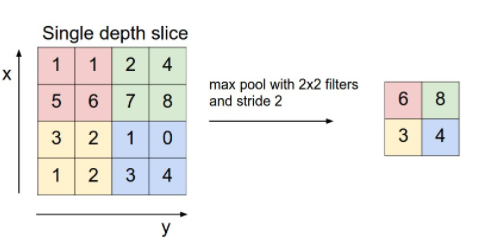
\includegraphics[width=.49\textwidth]{Plots/MaxPool.png}
\end{center}

Average pooling is similar except that you would take the average of each patch as its output instead of the maximum.

Consider the following 4 matrices:
$$
\begin{bmatrix}
    1 & 1 & 1 & 0 \\
    1 & 1 & 1 & 0 \\
    1 & 1 & 1 & 0 \\
    0 & 0 & 0 & 0
\end{bmatrix},
%
\begin{bmatrix}
    0 & 1 & 1 & 1 \\
    0 & 1 & 1 & 1 \\
    0 & 1 & 1 & 1 \\
    0 & 0 & 0 & 0
\end{bmatrix},
%
\begin{bmatrix}
    0 & 0 & 0 & 0 \\
    0 & 1 & 1 & 1 \\
    0 & 1 & 1 & 1 \\
    0 & 1 & 1 & 1
\end{bmatrix},
%
\begin{bmatrix}
    0 & 0 & 0 & 0 \\
    1 & 1 & 1 & 0 \\
    1 & 1 & 1 & 0 \\
    1 & 1 & 1 & 0
\end{bmatrix}
$$
\problem[3]

Apply $2 \times 2$ average pooling with a stride of 2 to each of the above images.

\begin{solution}

\[
    \begin{bmatrix}
        1 & 0.5\\
        0.5 & 0.25
    \end{bmatrix},
    %
    \begin{bmatrix}
        0.5 & 1\\
        0.25 & 0.5
    \end{bmatrix},
    %
    \begin{bmatrix}
        0.25 & 0.5\\
        0.5 & 1
    \end{bmatrix},
    %
    \begin{bmatrix}
        0.5 & 0.25\\
        1 & 0.5
    \end{bmatrix}
\]

\end{solution}

\problem[3]

Apply $2 \times 2$ max pooling with a stride of 2 to each of the above images.

\begin{solution}
    \[
    \begin{bmatrix}
        1 & 1\\
        1 & 1
    \end{bmatrix},
    %
    \begin{bmatrix}
        1 & 1\\
        1 & 1
    \end{bmatrix},
    %
    \begin{bmatrix}
        1 & 1\\
        1 & 1
    \end{bmatrix},
    %
    \begin{bmatrix}
        1 & 1\\
        1 & 1
    \end{bmatrix}
\]
\end{solution}

\problem[4]

Consider a scenario in which we wish to classify a dataset of images of various animals, where an animal may appear at various angles/locations of the image, and the image contains small amounts of noise (e.g. some pixels may be missing). Why might pooling be advantageous given these properties of our dataset?

\begin{solution}
    With pooling, the impact of individual pixels is lessened, since the values are pooled with adjacent pixels to eliminate outlier and noisy values. If one value is missing or an outlier, the nearby normal pixel values can correct for the outlier when pooling is performed, averaging out the noise. If the images are translated or rotated, key data may no longer be processed by the same weights in the neural network. However, with pooling, the same weights in the network are able to process nearby pixel data, since pooling captures information from a neighborhood of pixels. This makes the network robust to small rotations and translations.
\end{solution}

\newpage

\subsection{PyTorch implementation}
\problem[20]

Using PyTorch ``Sequential'' model class as you did in 2C, build a deep \emph{convolutional}
network to classify the handwritten digits in MNIST. You are now allowed to use
the following layers (but \textbf{only} the following):

 \begin{itemize}
    \item \textbf{Linear:} A fully-connected layer
    \begin{itemize}
        \item In convolutional networks, Linear (also called dense) layers are typically used to knit together higher-level feature representations.
        \item Particularly useful to map the 2D features resulting from the last convolutional layer to categories for classification (like the 1000 categories of ImageNet or the 10 categories of MNIST).
        \item Inefficient use of parameters and often overkill: for $A$ input activations and $B$ output activations, number of parameters needed scales as $O(AB)$.
    \end{itemize}
    \item \textbf{Conv2d:} A 2-dimensional convolutional layer
    \begin{itemize}
        \item The bread and butter of convolutional networks, conv layers impose a translational-invariance prior on a fully-connected network. By sliding filters across the image to form another image, conv layers perform ``coarse-graining'' of the image.
        \item Networking several convolutional layers in succession helps the convolutional network knit together more abstract representations of the input. As you go higher in a convolutional network, activations represent pixels, then edges, colors, and finally objects.
        \item More efficient use of parameters. For $N$ filters of $K \times K$ size on an input of size $L \times L$, the number of parameters needed scales as $O(N K^2)$. When $N, K$ are small, this can often beat the $O(L^4)$ scaling of a Linear layer applied to the $L^2$ pixels in the image.

    \end{itemize}
    \item \textbf{MaxPool2d:} A 2-dimensional max-pooling layer
    \begin{itemize}
        \item Another way of performing ``coarse-graining'' of images, max-pool layers are another way of ignoring finer-grained details by only considering maximum activations over small patches of the input.
        \item Drastically reduces the input size. Useful for reducing the number of parameters in your model.
        \item Typically used immediately following a series of convolutional-activation layers.
    \end{itemize}
    \item \textbf{BatchNorm2d:} Performs batch normalization (Ioffe and Szegedy, 2014). Normalizes the activations of previous layer to standard normal (mean 0, standard deviation 1).
    \begin{itemize}
        \item Accelerates convergence and improves performance of model, especially when saturating nonlinearities (sigmoid) are used.
        \item Makes model less sensitive to higher learning rates and initialization, and also acts as a form of regularization.
        \item Typically used immediately before nonlinearity (Activation) layers.
    \end{itemize}
    \item \textbf{Dropout:} Takes some probability and at every iteration sets weights to zero at random with that probability
    \begin{itemize}
        \item An effective form of regularization. During training, randomly selecting activations to shut off forces network to build in redundancies in the feature representation, so it does not rely on any single activation to perform classification.
    \end{itemize}
    \item \textbf{ReLU (activation):} Sets negative inputs to 0
    \item \textbf{Softmax (activation):} Rescales input so that it can be interpreted as a (discrete) probability distribution.
    \item \textbf{Flatten:} Flattens any tensor into a single vector (required in order to pass a 2D tensor output from a convolutional layer as input into Linear layers)
\end{itemize}

\textbf{Your tasks.} Build a network with only the allowed layers that achieves \textbf{test accuracy of at least 0.985}. You are required to use categorical cross entropy as your loss function and to train for 10 epochs with a batch size of 32. Note: your model must have fewer than 1 million parameters, as measured by the method given in the sample code.
Everything else can change: optimizer (e.g., RMSProp, Adam), initial learning rates, dropout probabilities, layerwise regularizer strengths, etc. You are not required to use all of the layers, but \emph{you must have
at least one dropout layer and one batch normalization layer in your final model}. Try to figure out the best possible architecture and hyperparameters given these building blocks!

In order to design your model, you should train your model for 1 epoch (batch size 32) and look at the final \textbf{test accuracy}  after training. This should take no more than 10 minutes, and should give you an immediate sense for how fast your network converges and how good it is.

Set the probabilities of your
dropout layers to 10 equally-spaced values $p \in [0, 1]$, train for 1 epoch, and report the final model accuracies for each.

You can perform all of your hyperparameter validation in this way: vary your parameters and train for an epoch. After you're satisfied with the model design, you should train your model for the full 10 epochs.

\textbf{In your submission.} Turn in the code of your model, the test accuracy for the 10 dropout probabilities $p \in [0, 1]$, and the
final test accuracy when your model
is trained for 10 epochs. We should have everything needed to reproduce your results.

Discuss what you found to be the most effective strategies in designing a convolutional network. Which regularization method was most effective (dropout, layerwise regularization, batch norm)?

Do you foresee any problem with this way of validating our hyperparameters? If so, why?

\emph{Hints:}

\begin{itemize}
    \item You are provided with a sample network that achieves a high accuracy. Starting with this network, modify some of the regularization parameters (layerwise regularization strength, dropout probabilities) to see if you can maximize the test accuracy. You can also add layers or modify layers (e.g.
    changing the convolutional kernel sizes, number of filters, stride, dilation, etc.) so long as the total number of parameters remains under the cap of 1 million.
    \item You may want to read up on successful convolutional architectures, and emulate some of their design principles. Please cite any idea you use that is not your own.
    \item To better understand the function of each layer, check the PyTorch documentation.
    \item Linear layers take in single vector inputs (ex: \emph{(784, )}) but Conv2D layers
    take in tensor inputs (ex: \emph{(28, 28, 1)}): width, height, and channels. Using the transformation \verb$transforms.ToTensor()$ when loading the dataset will reshape the training/test $X$ to a 4-dimensional tensor (ex: \emph{(num_examples, width, height, channels)}) and normalize values. For the MNIST dataset, \emph{channels=1}. Typical color images have 3 color channels, 1 for each color in RGB.
    \item If your model is running slowly on your CPU, try making each layer smaller
    and stacking more layers so you can leverage deeper representations.
    \item Other useful CNN design principles:
    \begin{itemize}
        \item CNNs perform well with many stacked convolutional layers, which develop increasingly large-scale representations of the input image.
        \item Dropout ensures that the learned representations are robust to some amount of noise.
        \item Batch norm is done after a convolutional or dense layer and immediately prior to an activation/nonlinearity layer.
        \item Max-pooling is typically done after a series of convolutions, in order to gradually reduce the size of the representation.
        \item Finally, the learned representation is passed into a dense layer (or two), and then filtered down to the final softmax layer.
    \end{itemize}
\end{itemize}

\newpage

\begin{solution}
    \href{https://colab.research.google.com/drive/1_5RHjUBimDTXiCALfpDKq3nsC0YWss3A?usp=sharing}{Code link}

    https://colab.research.google.com/drive/1_5RHjUBimDTXiCALfpDKq3nsC0YWss3A?usp=sharing

    Test error after 1 epoch for different dropout probabilities on all dropout layers:
    \begin{center}
        \begin{tabular}{|c|c|}
            \hline
            $p$ & Test accuracy\\
            \hline
            0 & 0.9842\\
            0.1 & 0.9831\\
            0.2 & 0.9803\\
            0.3 & 0.9764\\
            0.4 & 0.9665\\
            0.5 & 0.9484\\
            0.6 & 0.9156\\
            0.7 & 0.7674\\
            0.8 & 0.5509\\
            0.9 & 0.1148\\
            1 & 0.0924\\
            \hline  
        \end{tabular}
    \end{center}

    \begin{verbatim}
        model = nn.Sequential(
            nn.Conv2d(1, 16, kernel_size=5),
            nn.BatchNorm2d(16),
            nn.ReLU(),
            nn.MaxPool2d(2),
            nn.Dropout(p=0.1),
            
            nn.Conv2d(16, 32, kernel_size=3),
            nn.BatchNorm2d(32),
            nn.ReLU(),
            nn.MaxPool2d(2),
            nn.Dropout(p=0.1),
        
            nn.Conv2d(32, 32, kernel_size=3),
            nn.BatchNorm2d(32),
            nn.ReLU(),
            nn.MaxPool2d(2),
            nn.Dropout(p=0.1),
            
            nn.Flatten(),
            nn.Linear(32, 128),
            nn.ReLU(),
            nn.Linear(128, 10)
        )
    \end{verbatim}

    The designed model has 19978 model parameters, coming from 3 convolutional layers with batch norm and 2 linear layers.

    After training the model for 10 epochs with batch size 32 and learning rate 0.001 (default Adam), the model achieved a final validation (test) accuracy of $\boxed{0.9895}$.

    The most successful strategy in designing the CNN was to stack multiple 2D convolution layers, with only a few linear layers at the end. Additionally, the design principles of using batch norm prior to activation for each convolutional layer proved effective. Using dropout regularization after each convolutional layer also improved the model and reduced overfitting. However, generally higher dropout probabilities caused too much underfitting, so keeping $p$ low for dropout layers was the most effective design choice. Overall, batch norm regularization was more effective at reducing overfitting than dropout regularization.

    % Validation of hyperparameters by manually checking and testing each value is extremely slow and inefficient. Additionally, for hyperparameter values that are not bounded by some range (unlike dropout probability, which is bounded between 0 and 1), we must test different orders of magnitude for each hyperparameter. This leads to a multi-dimensional optimization problem that can be very difficult and time consuming to solve.

    By using only a single validation set to pick our hyperparameters, we risk overfitting the model to the specific validation set. We may end up picking a model that performs well on the validation set, but will do poorly on data out of sample. Thus it is unwise to estimate the test error using a validation set if that validation error is being used to optimize the model.
\end{solution}


\end{document}
